%% analyse.tex
%% $Id: analyse.tex 61 2012-05-03 13:58:03Z bless $
% !TEX root = thesis.tex

\chapter{Analyse und Evaluierung}
\label{ch:AnalyseUndEvaluierung}
%% ==============================

Die Beantwortung der Leitfrage des Projekts, ob durch Quantified Self das Wohlbefinden verbessert werden kann, hängt maßgeblich von einer genauen Analyse der Daten ab. 
Die zuvor in der Datengenerierungsphase erhobenen Daten müssen unter Berücksichtigung etwaiger Fremdeinflüsse bzw. Verfälschungen analysiert und ausgewertet werden.
Um dies zu gewährleisten sind wichtige Anforderungen an die Analyse gestellt, auf die im Folgenden näher eingegangen wird.

Exemplarische wurden nun nachdem alle Daten analysiert und ausgewertet wurden eine Testperson ausgewählt, anhand der die Leitfrage „Lässt sich das Wohlbefinden durch Quantified Self verbessern?“ beantwortet werden soll.
Diese soll mit Hilfe von zwei weiteren Fragen beantwortet werden.

\begin{itemize}
	\item Wie hängt die Anzahl der Schritte pro Tag mit der Schlafqualität zusammen und wie beeinflusst Sport diesen? 
	\item Welchen Einfluss hat die Schlafqualität auf die tägliche Stimmung?
\end{itemize}

Aufgrund einer in der Gesamtheit Neuerhebung von Daten, liegt bei deren Auswertung der Fokus auf der deskriptive Datenanalyse.

\begin{quote}
\textit{„Deskriptive Datenanalyse: Liegt eine Totalerhebung oder generell ein Datensatz vor, so ist es die Aufgabe der Datenanalyse, die in den Einzeldaten enthaltene Information zu verdichten und diese so darzustellen, dass Wesentliches deutlich wird. Dazu werden Tabellen, graphische Darstellungen und charakteristische Maßzahlen verwendet.  Die Datenanalyse hat ausschließlich beschreibenden Charakter (deskriptive Statistik).“} 
\end{quote}
\cite[Springer Gabler Wirtschaftslexikon]{web:SpringerDatenanalyse}

Laut Schäfer\cite{Schafer2010} ist im Anschluss der deskriptiven Datenanalye mit der explorativen Statistik fortzufahren.
Dabei wird versucht Muster zu erkennen, welche mit Hilfe von Grafiken und Daten beschrieben werden.
Abschließend wird mit der Inferenzstatistik die Auswertung vollendet.
In diesem letzten Schritt wird versucht mit Hilfe von Stichprobendaten auf die allgemeine These zu schließen.
\\
\\
%Dazu wurden verschiedene Korrelationskoeffizienten berechnet und Graphen erstellt.

%% ==============================
\section{Anzahl der Schritte, Schlafqualität und\\ Energieverbrauch}
%% ==============================
\label{ch:AnalyseUndEvaluierung:sec:SchritteSchlafqualitätUndEnergieverbrauch}


Das Diagramm \ref{fig:SchritteSchlafqualitätUndEnergieverbrauch} zeigt die Anzahl der aufgenommen Schritte pro Tag und zusätzlich die Schlafqualität in Prozent des jeweiligen Tages. \\
Außerdem zeigt das Diagramm den Energieverbrauch des jeweiligen Aufzeichnungstages in Kilokalorien an.
Diese Daten können zusätzlich \marginpar{noch zu beschrieben in "Moves Section"}in der Applikation Moves angegeben werden[\ref{ch:Apps:sec:Hueman:subsec:DuFe}]. \\ 
Die Werte der Grafik beziehen sich auf den kompletten Aufzeichnugszeitraums. 
Dabei handelt es sich bei den grünen Punkten um die einzelnen Datenpunkte der Schlafqualität, welche in Prozent auf der rechten Abzissenachse angegeben ist.
Auf der linken Abzissenachse wiederum wird die gesamte Anzahl der Schritte in blauen Punkten gezeigt, wie es auch der Legende zu entnehmen ist. \\
Zur besser Trend Ersichtlichkeit sind alle Datenreihen zusätzlich in einem Polynom sechsten Grades angenähert und linear dargestellt.
Diese Werte sind über den Erhebungszeitraum dargestellt. \\
In der Abbildung kommen die Werte „Schritte pro Tag” aus der im Projekt verwendeten Applikation Moves[\ref{ch:Apps:sec:Moves}]. 
Sleep Cycle[\ref{ch:Apps:sec:SleepCycle}] liefert dabei die Daten zur Schlafqualität.
Die Werte wurden im Zuge des Projektes von den Autoren im Monat Mai des Jahres 2014 erhoben. \\
Über den gesamten Aufzeichnungsraum ist der Energieverbrauch nahezu gleichbleibend, nur gegen Ende steigt die sportliche Aktivität leicht an.
Es ist zu erkennen, dass die Basiswerte der Anzahl der Schritte pro Tag im Zeitraum vom 11.05 bis zum 26.05 leicht fallen und zum Ende hin wieder zunehmen. 
Vom Anfang der Erhebungsphase bis zum 08.05 etwa steigt die Anzahl der Schritte pro Tag zu etwa 6000. \\
Zusätzlich ist zu sagen, dass einige Werte über 90\% unter dem Durchschnitt liegen.
Der Durchschnitt der Schlafqualität über den ausgewählten Zeitraum ist 78\%.
Während der ersten Woche sinkt die Schlafqualität bis auf unter 70\% Punkten.
Danach stagnieren die Werte bis zum 25.05 um gegen Ende der Datenerhebungsphase auf 100\% anzusteigen.
\\
Gesteigerte Laufaktivität scheint nicht mit einem verbesserten Schlaf belohnt zu werden, ebenso müsste die Testperson weniger Sport betreiben um eine bessere Schlafqualität zu erreichen.
Deutlich wird dies im Zeitraum vom 21.05 bis zum 26.05. 
Während der Energieverbrauch steigt, sinkt die Schlafqualität.
Hier stellt sich die Frage, ob die Hard- bzw. Software falsche Daten liefern oder es scheinbar wirklich so ist, wie es aussieht.
Zu beachten ist das Kapitel Relativierung[\ref{ch:Relativierung}].

\begin{figure}[H]
\centering
        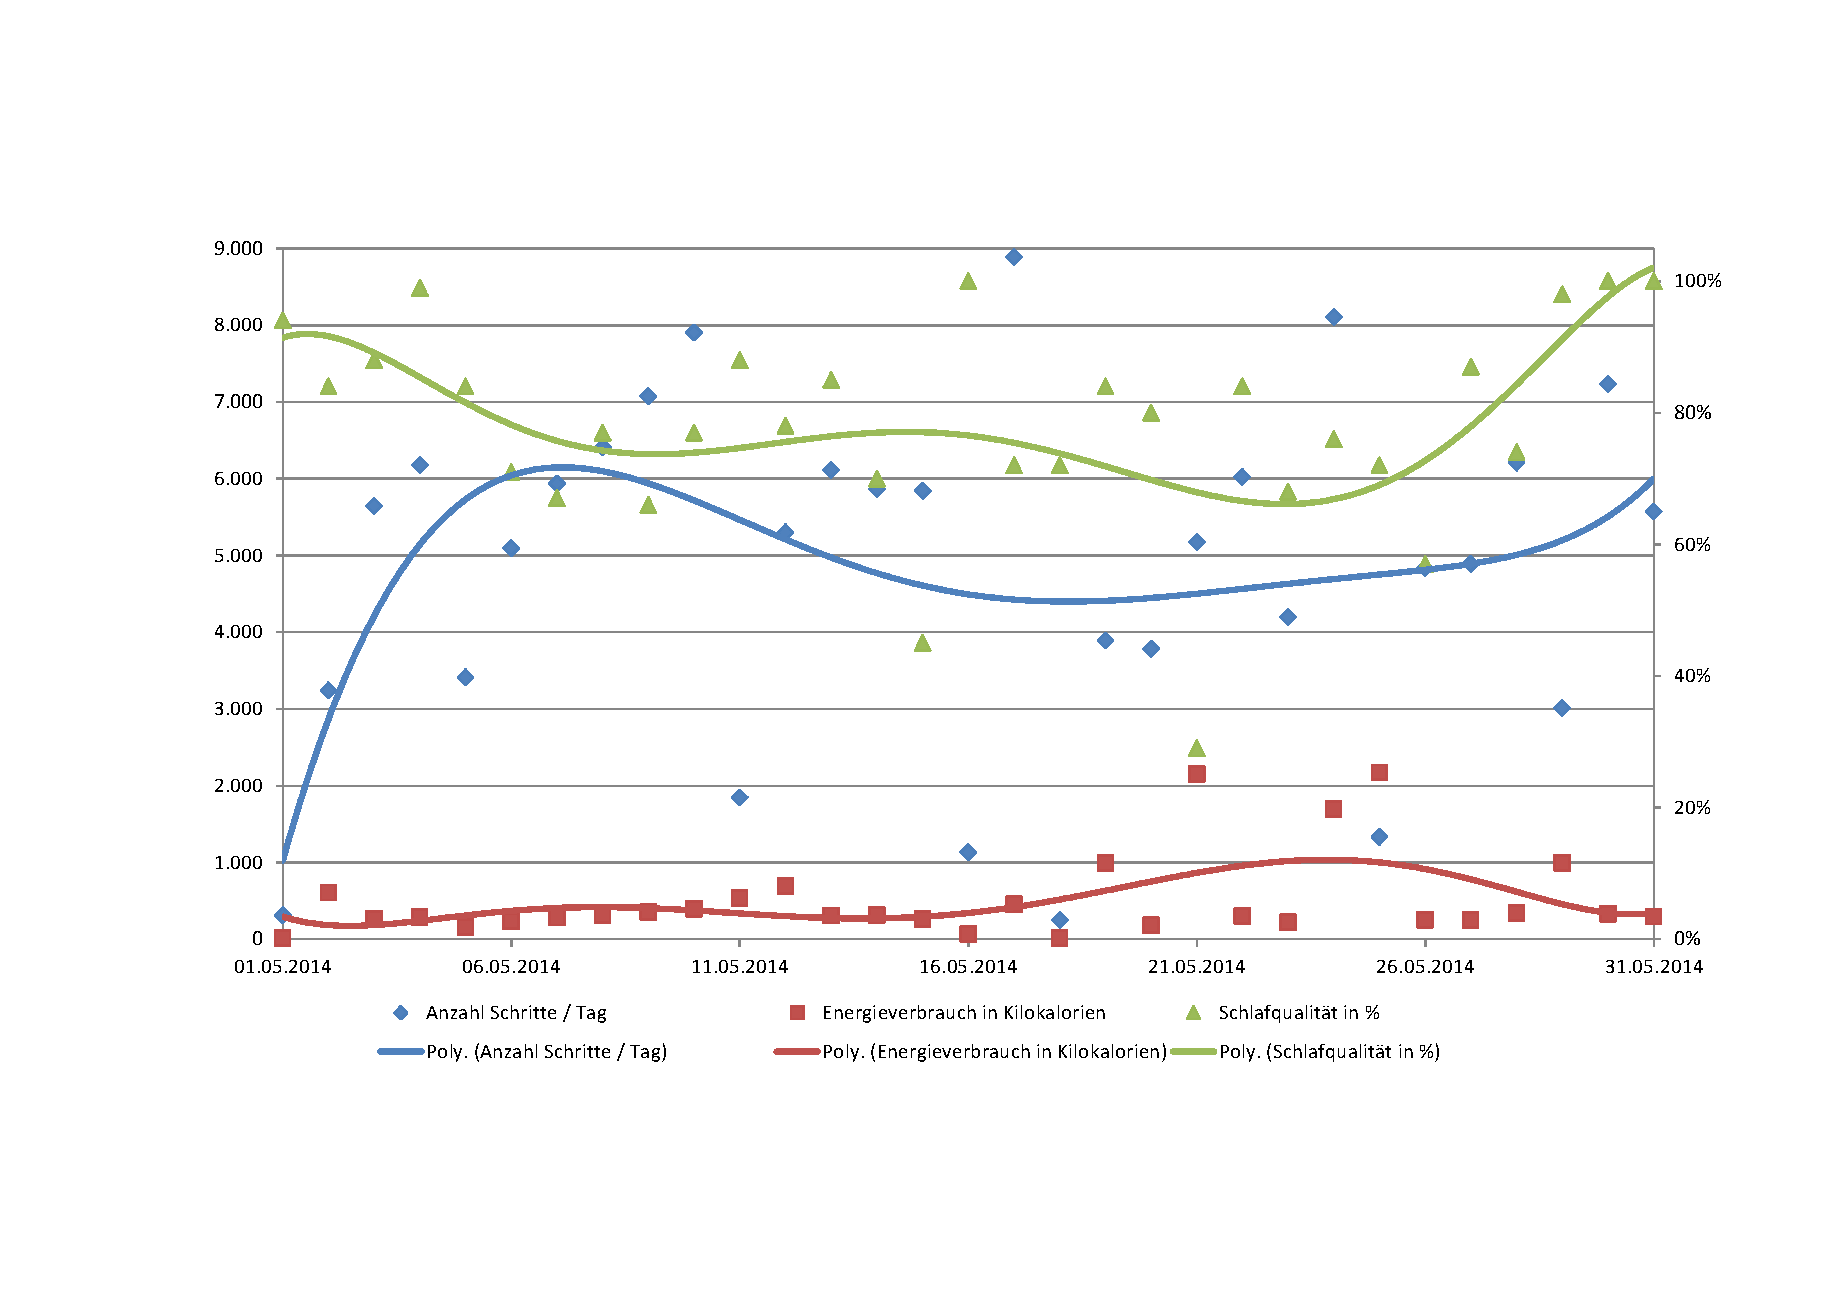
\includegraphics[angle=270,width=0.9\textwidth]{images/Analyse/Sleep-Steps-kcal} 
        \caption[Daten der Schritte pro Tag, der Schlafqualität und des Energieverbrauchs]{Daten der Schritte pro Tag, der Schlafqualität und des Energieverbrauchs}
        \label{fig:SchritteSchlafqualitätUndEnergieverbrauch}
\end{figure}


%% ==============================
\section{Schlafqualität und Stimmung}
%% ==============================
\label{ch:AnalyseUndEvaluierung:sec:SchlafqualitätUndStimmung}

Bei der im Diagramm [\ref{fig:SchlafqualitätUndStimmung}] in grün dargestellten Datenpunkte handelt es sich um die gleichen Werte wie im Kapitel \ref{ch:AnalyseUndEvaluierung:sec:SchritteSchlafqualitätUndEnergieverbrauch} beschrieben. 
Die Quelle ist ebenfalls die wie vorher beschrieben die Gleiche.
Die Abbildung \ref{fig:SchlafqualitätUndStimmung} zeigt den zuvor beschriebenen Graphen und den Stimmungsverlauf über den Datenerhebungszeitraum in der Farbe Orange.
Die rechte Abzissenachse zeigt die Stimmung auf einer Skala von eins bis drei, wobei drei ein gutes Wohlbefinden heißt, zwei ein neutrales und eins ein schlechtes.

\begin{figure}[H]
\centering
        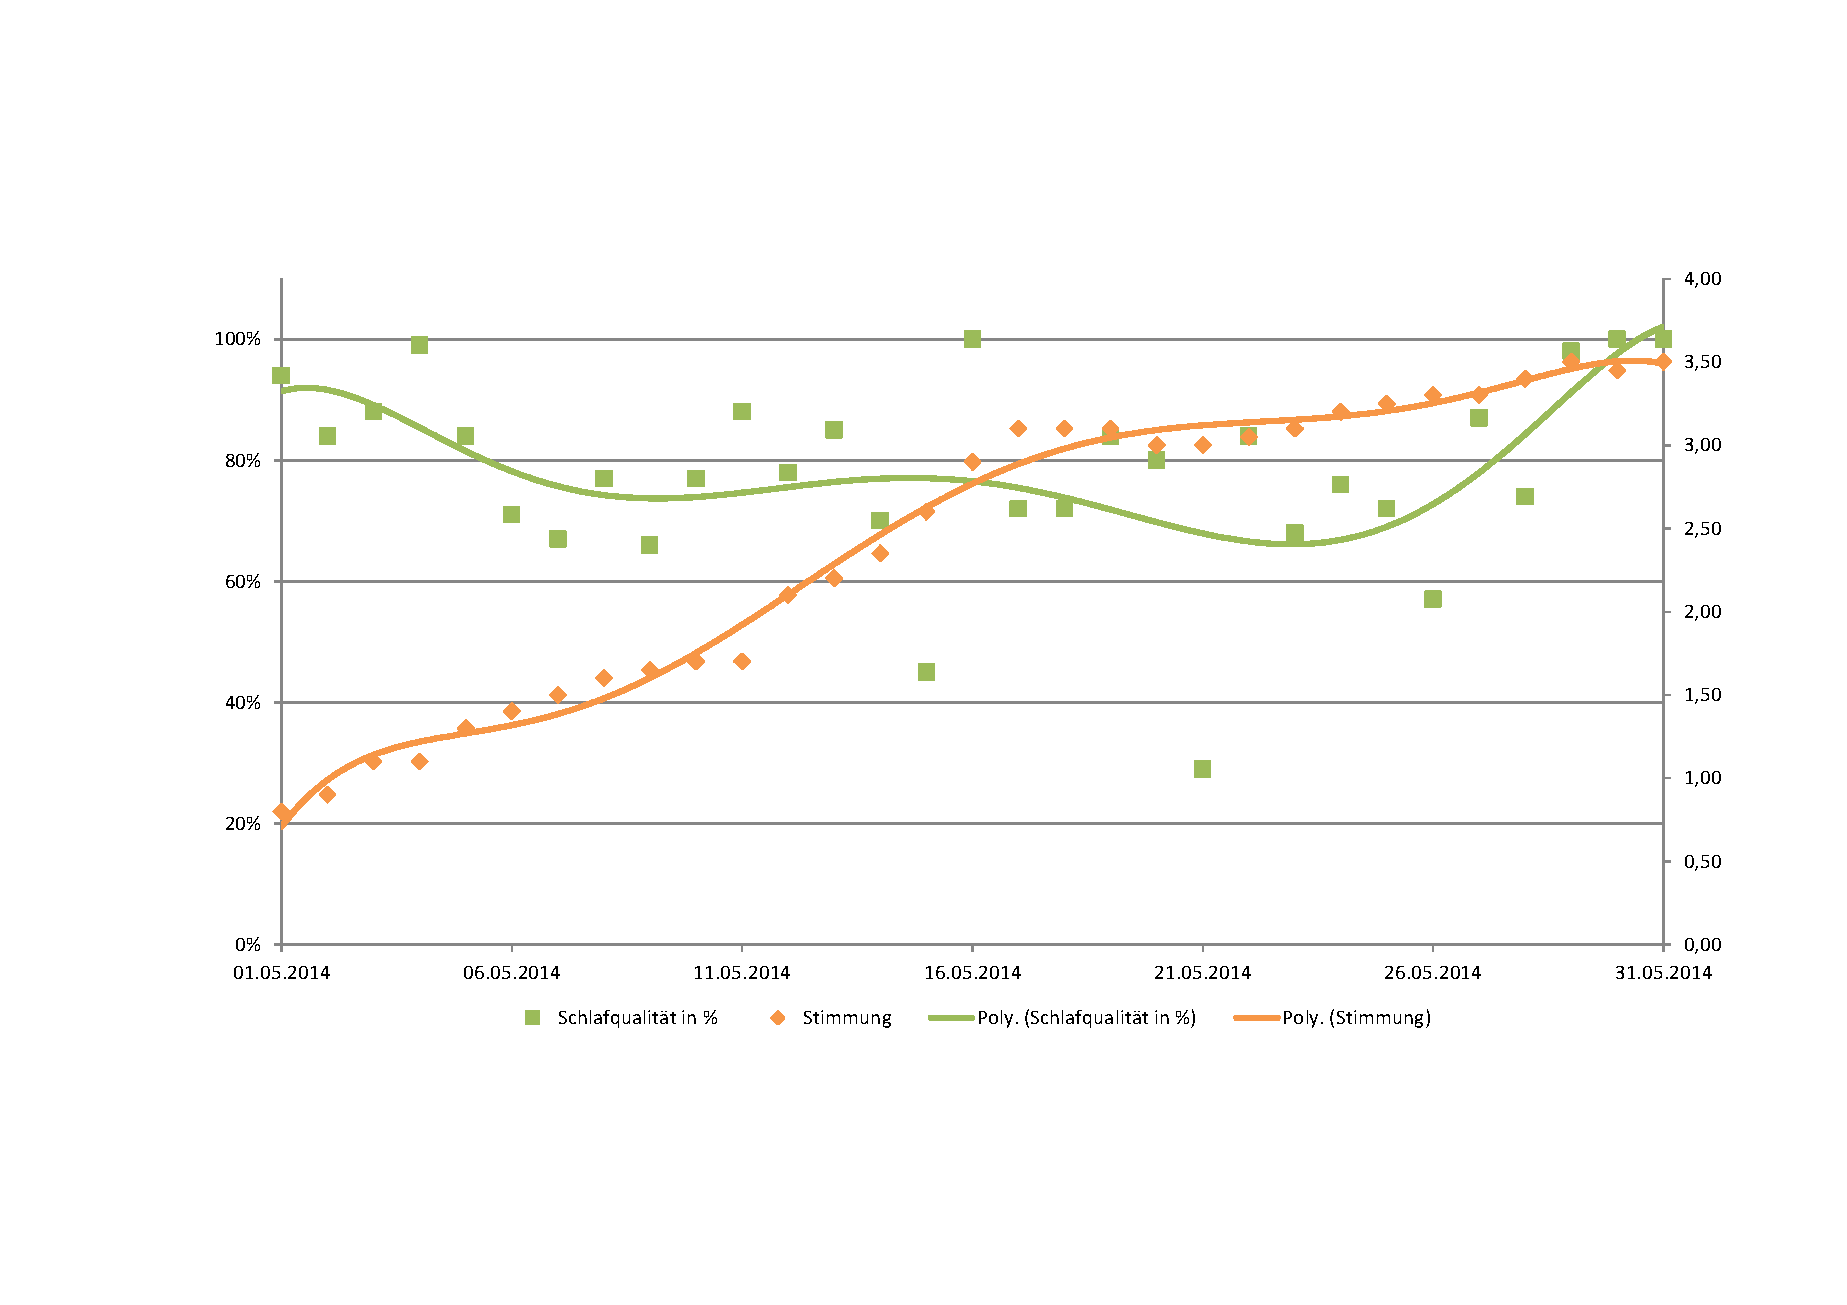
\includegraphics[angle=270,width=0.8\textwidth]{images/Analyse/Sleep-Mood} 
        \caption[Daten der Stimmung und Schlafqualität]{Daten der Stimmung und Schlafqualität}
        \label{fig:SchlafqualitätUndStimmung}
\end{figure}

%% inferenzstatistik kann => nicht applyable weil nicht repräsentativ, referenzieren auf relativierung

%%% Local Variables: 
%%% mode: latex
%%% TeX-master: "thesis"
%%% End: 
